\documentclass[]{article}
\usepackage{lmodern}
\usepackage{amssymb,amsmath}
\usepackage{ifxetex,ifluatex}
\usepackage{fixltx2e} % provides \textsubscript
\ifnum 0\ifxetex 1\fi\ifluatex 1\fi=0 % if pdftex
  \usepackage[T1]{fontenc}
  \usepackage[utf8]{inputenc}
\else % if luatex or xelatex
  \ifxetex
    \usepackage{mathspec}
  \else
    \usepackage{fontspec}
  \fi
  \defaultfontfeatures{Ligatures=TeX,Scale=MatchLowercase}
\fi
% use upquote if available, for straight quotes in verbatim environments
\IfFileExists{upquote.sty}{\usepackage{upquote}}{}
% use microtype if available
\IfFileExists{microtype.sty}{%
\usepackage{microtype}
\UseMicrotypeSet[protrusion]{basicmath} % disable protrusion for tt fonts
}{}
\usepackage[margin=1in]{geometry}
\usepackage{hyperref}
\hypersetup{unicode=true,
            pdftitle={Eksploracja Masywnych Danych - Analiza danych},
            pdfauthor={Kajetan Zimniak \& Bartosz Górka},
            pdfborder={0 0 0},
            breaklinks=true}
\urlstyle{same}  % don't use monospace font for urls
\usepackage{color}
\usepackage{fancyvrb}
\newcommand{\VerbBar}{|}
\newcommand{\VERB}{\Verb[commandchars=\\\{\}]}
\DefineVerbatimEnvironment{Highlighting}{Verbatim}{commandchars=\\\{\}}
% Add ',fontsize=\small' for more characters per line
\usepackage{framed}
\definecolor{shadecolor}{RGB}{248,248,248}
\newenvironment{Shaded}{\begin{snugshade}}{\end{snugshade}}
\newcommand{\AlertTok}[1]{\textcolor[rgb]{0.94,0.16,0.16}{#1}}
\newcommand{\AnnotationTok}[1]{\textcolor[rgb]{0.56,0.35,0.01}{\textbf{\textit{#1}}}}
\newcommand{\AttributeTok}[1]{\textcolor[rgb]{0.77,0.63,0.00}{#1}}
\newcommand{\BaseNTok}[1]{\textcolor[rgb]{0.00,0.00,0.81}{#1}}
\newcommand{\BuiltInTok}[1]{#1}
\newcommand{\CharTok}[1]{\textcolor[rgb]{0.31,0.60,0.02}{#1}}
\newcommand{\CommentTok}[1]{\textcolor[rgb]{0.56,0.35,0.01}{\textit{#1}}}
\newcommand{\CommentVarTok}[1]{\textcolor[rgb]{0.56,0.35,0.01}{\textbf{\textit{#1}}}}
\newcommand{\ConstantTok}[1]{\textcolor[rgb]{0.00,0.00,0.00}{#1}}
\newcommand{\ControlFlowTok}[1]{\textcolor[rgb]{0.13,0.29,0.53}{\textbf{#1}}}
\newcommand{\DataTypeTok}[1]{\textcolor[rgb]{0.13,0.29,0.53}{#1}}
\newcommand{\DecValTok}[1]{\textcolor[rgb]{0.00,0.00,0.81}{#1}}
\newcommand{\DocumentationTok}[1]{\textcolor[rgb]{0.56,0.35,0.01}{\textbf{\textit{#1}}}}
\newcommand{\ErrorTok}[1]{\textcolor[rgb]{0.64,0.00,0.00}{\textbf{#1}}}
\newcommand{\ExtensionTok}[1]{#1}
\newcommand{\FloatTok}[1]{\textcolor[rgb]{0.00,0.00,0.81}{#1}}
\newcommand{\FunctionTok}[1]{\textcolor[rgb]{0.00,0.00,0.00}{#1}}
\newcommand{\ImportTok}[1]{#1}
\newcommand{\InformationTok}[1]{\textcolor[rgb]{0.56,0.35,0.01}{\textbf{\textit{#1}}}}
\newcommand{\KeywordTok}[1]{\textcolor[rgb]{0.13,0.29,0.53}{\textbf{#1}}}
\newcommand{\NormalTok}[1]{#1}
\newcommand{\OperatorTok}[1]{\textcolor[rgb]{0.81,0.36,0.00}{\textbf{#1}}}
\newcommand{\OtherTok}[1]{\textcolor[rgb]{0.56,0.35,0.01}{#1}}
\newcommand{\PreprocessorTok}[1]{\textcolor[rgb]{0.56,0.35,0.01}{\textit{#1}}}
\newcommand{\RegionMarkerTok}[1]{#1}
\newcommand{\SpecialCharTok}[1]{\textcolor[rgb]{0.00,0.00,0.00}{#1}}
\newcommand{\SpecialStringTok}[1]{\textcolor[rgb]{0.31,0.60,0.02}{#1}}
\newcommand{\StringTok}[1]{\textcolor[rgb]{0.31,0.60,0.02}{#1}}
\newcommand{\VariableTok}[1]{\textcolor[rgb]{0.00,0.00,0.00}{#1}}
\newcommand{\VerbatimStringTok}[1]{\textcolor[rgb]{0.31,0.60,0.02}{#1}}
\newcommand{\WarningTok}[1]{\textcolor[rgb]{0.56,0.35,0.01}{\textbf{\textit{#1}}}}
\usepackage{longtable,booktabs}
\usepackage{graphicx,grffile}
\makeatletter
\def\maxwidth{\ifdim\Gin@nat@width>\linewidth\linewidth\else\Gin@nat@width\fi}
\def\maxheight{\ifdim\Gin@nat@height>\textheight\textheight\else\Gin@nat@height\fi}
\makeatother
% Scale images if necessary, so that they will not overflow the page
% margins by default, and it is still possible to overwrite the defaults
% using explicit options in \includegraphics[width, height, ...]{}
\setkeys{Gin}{width=\maxwidth,height=\maxheight,keepaspectratio}
\IfFileExists{parskip.sty}{%
\usepackage{parskip}
}{% else
\setlength{\parindent}{0pt}
\setlength{\parskip}{6pt plus 2pt minus 1pt}
}
\setlength{\emergencystretch}{3em}  % prevent overfull lines
\providecommand{\tightlist}{%
  \setlength{\itemsep}{0pt}\setlength{\parskip}{0pt}}
\setcounter{secnumdepth}{0}
% Redefines (sub)paragraphs to behave more like sections
\ifx\paragraph\undefined\else
\let\oldparagraph\paragraph
\renewcommand{\paragraph}[1]{\oldparagraph{#1}\mbox{}}
\fi
\ifx\subparagraph\undefined\else
\let\oldsubparagraph\subparagraph
\renewcommand{\subparagraph}[1]{\oldsubparagraph{#1}\mbox{}}
\fi

%%% Use protect on footnotes to avoid problems with footnotes in titles
\let\rmarkdownfootnote\footnote%
\def\footnote{\protect\rmarkdownfootnote}

%%% Change title format to be more compact
\usepackage{titling}

% Create subtitle command for use in maketitle
\providecommand{\subtitle}[1]{
  \posttitle{
    \begin{center}\large#1\end{center}
    }
}

\setlength{\droptitle}{-2em}

  \title{Eksploracja Masywnych Danych - Analiza danych}
    \pretitle{\vspace{\droptitle}\centering\huge}
  \posttitle{\par}
    \author{Kajetan Zimniak \& Bartosz Górka}
    \preauthor{\centering\large\emph}
  \postauthor{\par}
      \predate{\centering\large\emph}
  \postdate{\par}
    \date{27 October, 2019}


\begin{document}
\maketitle

{
\setcounter{tocdepth}{2}
\tableofcontents
}
\hypertarget{podsumowanie-analizy}{%
\section{Podsumowanie analizy}\label{podsumowanie-analizy}}

TODO: Podsumowanie na koniec

\hypertarget{wykorzystane-biblioteki}{%
\section{Wykorzystane biblioteki}\label{wykorzystane-biblioteki}}

\begin{itemize}
\tightlist
\item
  \texttt{knitr}
\item
  \texttt{dplyr}
\item
  \texttt{tidyverse}
\item
  \texttt{ggplot2}
\item
  \texttt{gridExtra}
\end{itemize}

\hypertarget{ustawienie-ziarna-generatora}{%
\section{Ustawienie ziarna
generatora}\label{ustawienie-ziarna-generatora}}

Celem zapewnienia powtarzalności operacji losowania, a co za tym idzie
powtarzalności wyników przy każdym uruchomieniu raportu na tych samych
danych zastosowano ziarno generatora o wartości \texttt{102019}.

\begin{Shaded}
\begin{Highlighting}[]
\KeywordTok{set.seed}\NormalTok{(}\DecValTok{102019}\NormalTok{)}
\end{Highlighting}
\end{Shaded}

\hypertarget{charakterystyka-obserwacji---zastosowane-atrybuty}{%
\section{Charakterystyka obserwacji - zastosowane
atrybuty}\label{charakterystyka-obserwacji---zastosowane-atrybuty}}

W ramach analizy mamy do czynienia z obserwacjami opisanymi za pomocą
następujących atrybutów:

\begin{itemize}
\tightlist
\item
  \textbf{length}: długość złowionego śledzia {[}cm{]}
\item
  \textbf{cfin1}: dostępność planktonu {[}zagęszczenie \emph{Calanus
  finmarchicus} gat. 1{]}
\item
  \textbf{cfin2}: dostępność planktonu {[}zagęszczenie \emph{Calanus
  finmarchicus} gat. 2{]};
\item
  \textbf{chel1}: dostępność planktonu {[}zagęszczenie \emph{Calanus
  helgolandicus} gat. 1{]};
\item
  \textbf{chel2}: dostępność planktonu {[}zagęszczenie \emph{Calanus
  helgolandicus} gat. 2{]};
\item
  \textbf{lcop1}: dostępność planktonu {[}zagęszczenie \emph{widłonogów}
  gat. 1{]};
\item
  \textbf{lcop2}: dostępność planktonu {[}zagęszczenie \emph{widłonogów}
  gat. 2{]};
\item
  \textbf{fbar}: natężenie połowów w regionie {[}ułamek pozostawionego
  narybku{]};
\item
  \textbf{recr}: roczny narybek {[}liczba śledzi{]};
\item
  \textbf{cumf}: łączne roczne natężenie połowów w regionie {[}ułamek
  pozostawionego narybku{]};
\item
  \textbf{totaln}: łączna liczba ryb złowionych w ramach połowu
  {[}liczba śledzi{]};
\item
  \textbf{sst}: temperatura przy powierzchni wody {[}°C{]};
\item
  \textbf{sal}: poziom zasolenia wody {[}Knudsen ppt{]};
\item
  \textbf{xmonth}: miesiąc połowu {[}numer miesiąca{]};
\item
  \textbf{nao}: oscylacja północnoatlantycka {[}mb{]}.
\end{itemize}

\hypertarget{wczytanie-danych-z-pliku}{%
\section{Wczytanie danych z pliku}\label{wczytanie-danych-z-pliku}}

Dane zamieszczone na stronie przedmiotu w postaci pliku CSV pobieramy
wyłącznie w sytuacji braku pliku w katalogu roboczym. Pozwala to nam na
ograniczenie niepotrzebnego transferu danych, jeżeli plik już istnieje.

\begin{Shaded}
\begin{Highlighting}[]
\NormalTok{file_name =}\StringTok{ "sledzie.csv"}
\NormalTok{source_url =}\StringTok{ "http://www.cs.put.poznan.pl/alabijak/emd/projekt/sledzie.csv"}

\ControlFlowTok{if}\NormalTok{ (}\OperatorTok{!}\KeywordTok{file.exists}\NormalTok{(file_name)) \{}
  \KeywordTok{download.file}\NormalTok{(source_url, }\DataTypeTok{destfile =}\NormalTok{ file_name, }\DataTypeTok{method =} \StringTok{"wget"}\NormalTok{)}
\NormalTok{\}}
\end{Highlighting}
\end{Shaded}

Po ewentualnym pobraniu wczytujemy dane do pamięci.

\begin{Shaded}
\begin{Highlighting}[]
\KeywordTok{library}\NormalTok{(}\StringTok{'knitr'}\NormalTok{)}
\KeywordTok{library}\NormalTok{(}\StringTok{'dplyr'}\NormalTok{)}
\KeywordTok{library}\NormalTok{(}\StringTok{'tidyverse'}\NormalTok{)}

\NormalTok{content =}
\StringTok{  }\NormalTok{file_name }\OperatorTok
\StringTok{  }\KeywordTok{read_csv}\NormalTok{(}\DataTypeTok{col_names =} \OtherTok{TRUE}\NormalTok{, }\DataTypeTok{na =} \KeywordTok{c}\NormalTok{(}\StringTok{""}\NormalTok{, }\StringTok{"NA"}\NormalTok{, }\StringTok{"?"}\NormalTok{)) }\OperatorTok
\StringTok{  }\KeywordTok{select}\NormalTok{(}\OperatorTok{-}\DecValTok{1}\NormalTok{)}

\NormalTok{content[}\DecValTok{0}\OperatorTok{:}\DecValTok{11}\NormalTok{] }\OperatorTok
\StringTok{  }\KeywordTok{head}\NormalTok{(}\DataTypeTok{n =} \DecValTok{5}\NormalTok{) }\OperatorTok
\StringTok{  }\KeywordTok{kable}\NormalTok{(}\DataTypeTok{align =} \StringTok{'c'}\NormalTok{, }\DataTypeTok{caption =} \StringTok{'Wybrane pomiary'}\NormalTok{)}
\end{Highlighting}
\end{Shaded}

\begin{longtable}[]{@{}ccccccccccc@{}}
\caption{Wybrane pomiary}\tabularnewline
\toprule
length & cfin1 & cfin2 & chel1 & chel2 & lcop1 & lcop2 & fbar & recr &
cumf & totaln\tabularnewline
\midrule
\endfirsthead
\toprule
length & cfin1 & cfin2 & chel1 & chel2 & lcop1 & lcop2 & fbar & recr &
cumf & totaln\tabularnewline
\midrule
\endhead
23.0 & 0.02778 & 0.27785 & 2.46875 & NA & 2.54787 & 26.35881 & 0.356 &
482831 & 0.3059879 & 267380.8\tabularnewline
22.5 & 0.02778 & 0.27785 & 2.46875 & 21.43548 & 2.54787 & 26.35881 &
0.356 & 482831 & 0.3059879 & 267380.8\tabularnewline
25.0 & 0.02778 & 0.27785 & 2.46875 & 21.43548 & 2.54787 & 26.35881 &
0.356 & 482831 & 0.3059879 & 267380.8\tabularnewline
25.5 & 0.02778 & 0.27785 & 2.46875 & 21.43548 & 2.54787 & 26.35881 &
0.356 & 482831 & 0.3059879 & 267380.8\tabularnewline
24.0 & 0.02778 & 0.27785 & 2.46875 & 21.43548 & 2.54787 & 26.35881 &
0.356 & 482831 & 0.3059879 & 267380.8\tabularnewline
\bottomrule
\end{longtable}

Oryginalnie zbiór posiada znaki \texttt{?} jako oznaczenie wartości
pustej (brakującej). Dzięki wykorzystaniu parametru \texttt{na} podczas
wywołania funkcji \texttt{read\_csv} możemy zastąpić znak \texttt{?}
poprawnym oznaczeniem braku wartości \texttt{NA}. W tabeli
\texttt{Wybrane\ pomiary} zaprezentowano pierwsze pięć obserwacji.

\hypertarget{podstawowe-statystyki-zbioru-danych}{%
\section{Podstawowe statystyki zbioru
danych}\label{podstawowe-statystyki-zbioru-danych}}

\begin{Shaded}
\begin{Highlighting}[]
\NormalTok{total_records =}\StringTok{ }\KeywordTok{count}\NormalTok{(content)}
\NormalTok{total_records_without_na_values =}\StringTok{ }\KeywordTok{count}\NormalTok{(}\KeywordTok{na.omit}\NormalTok{(content))}
\end{Highlighting}
\end{Shaded}

W zbiorze danych mamy do czynienia z 52582 obserwacjami opisanych za
pomocą 15 atrybutów. W całym zbiorze mamy do czynienia z 42488
obserwacjami bez wartości pustych co stanowi 81 procent całego zbioru.

\hypertarget{statystyka-parametruxf3w-obserwacji}{%
\subsection{Statystyka parametrów
obserwacji}\label{statystyka-parametruxf3w-obserwacji}}

\begin{Shaded}
\begin{Highlighting}[]
\NormalTok{content }\OperatorTok
\StringTok{  }\KeywordTok{summary}\NormalTok{() }\OperatorTok
\StringTok{  }\KeywordTok{kable}\NormalTok{(}\DataTypeTok{align =} \StringTok{'c'}\NormalTok{, }\DataTypeTok{caption =} \StringTok{'Statystyka zbioru danych'}\NormalTok{)}
\end{Highlighting}
\end{Shaded}

\begin{longtable}[]{@{}lccccccccccccccc@{}}
\caption{Statystyka zbioru danych}\tabularnewline
\toprule
& length & cfin1 & cfin2 & chel1 & chel2 & lcop1 & lcop2 & fbar & recr &
cumf & totaln & sst & sal & xmonth & nao\tabularnewline
\midrule
\endfirsthead
\toprule
& length & cfin1 & cfin2 & chel1 & chel2 & lcop1 & lcop2 & fbar & recr &
cumf & totaln & sst & sal & xmonth & nao\tabularnewline
\midrule
\endhead
& Min. :19.0 & Min. : 0.0000 & Min. : 0.0000 & Min. : 0.000 & Min. :
5.238 & Min. : 0.3074 & Min. : 7.849 & Min. :0.0680 & Min. : 140515 &
Min. :0.06833 & Min. : 144137 & Min. :12.77 & Min. :35.40 & Min. : 1.000
& Min. :-4.89000\tabularnewline
& 1st Qu.:24.0 & 1st Qu.: 0.0000 & 1st Qu.: 0.2778 & 1st Qu.: 2.469 &
1st Qu.:13.427 & 1st Qu.: 2.5479 & 1st Qu.:17.808 & 1st Qu.:0.2270 & 1st
Qu.: 360061 & 1st Qu.:0.14809 & 1st Qu.: 306068 & 1st Qu.:13.60 & 1st
Qu.:35.51 & 1st Qu.: 5.000 & 1st Qu.:-1.89000\tabularnewline
& Median :25.5 & Median : 0.1111 & Median : 0.7012 & Median : 5.750 &
Median :21.673 & Median : 7.0000 & Median :24.859 & Median :0.3320 &
Median : 421391 & Median :0.23191 & Median : 539558 & Median :13.86 &
Median :35.51 & Median : 8.000 & Median : 0.20000\tabularnewline
& Mean :25.3 & Mean : 0.4458 & Mean : 2.0248 & Mean :10.006 & Mean
:21.221 & Mean : 12.8108 & Mean :28.419 & Mean :0.3304 & Mean : 520366 &
Mean :0.22981 & Mean : 514973 & Mean :13.87 & Mean :35.51 & Mean : 7.258
& Mean :-0.09236\tabularnewline
& 3rd Qu.:26.5 & 3rd Qu.: 0.3333 & 3rd Qu.: 1.7936 & 3rd Qu.:11.500 &
3rd Qu.:27.193 & 3rd Qu.: 21.2315 & 3rd Qu.:37.232 & 3rd Qu.:0.4560 &
3rd Qu.: 724151 & 3rd Qu.:0.29803 & 3rd Qu.: 730351 & 3rd Qu.:14.16 &
3rd Qu.:35.52 & 3rd Qu.: 9.000 & 3rd Qu.: 1.63000\tabularnewline
& Max. :32.5 & Max. :37.6667 & Max. :19.3958 & Max. :75.000 & Max.
:57.706 & Max. :115.5833 & Max. :68.736 & Max. :0.8490 & Max. :1565890 &
Max. :0.39801 & Max. :1015595 & Max. :14.73 & Max. :35.61 & Max. :12.000
& Max. : 5.08000\tabularnewline
& NA & NA's :1581 & NA's :1536 & NA's :1555 & NA's :1556 & NA's :1653 &
NA's :1591 & NA & NA & NA & NA & NA's :1584 & NA & NA &
NA\tabularnewline
TODO: & Poprawić tabelk & ę, nie mieści się n & a stronie PDF & & & & &
& & & & & & &\tabularnewline
\bottomrule
\end{longtable}

\hypertarget{rozkux142ad-wartoux15bci-cech}{%
\subsection{Rozkład wartości cech}\label{rozkux142ad-wartoux15bci-cech}}

\begin{Shaded}
\begin{Highlighting}[]
\KeywordTok{library}\NormalTok{(}\StringTok{'ggplot2'}\NormalTok{)}
\KeywordTok{library}\NormalTok{(}\StringTok{'gridExtra'}\NormalTok{)}

\KeywordTok{ggplot}\NormalTok{(content, }\KeywordTok{aes}\NormalTok{(}\DataTypeTok{x =}\NormalTok{ length)) }\OperatorTok{+}\StringTok{ }\KeywordTok{geom_histogram}\NormalTok{(}\DataTypeTok{binwidth =} \FloatTok{0.25}\NormalTok{) }\OperatorTok{+}\StringTok{ }
\StringTok{  }\KeywordTok{theme_bw}\NormalTok{() }\OperatorTok{+}\StringTok{ }\KeywordTok{ggtitle}\NormalTok{(}\StringTok{'Długość złowionego śledzia [cm]'}\NormalTok{) }\OperatorTok{+}\StringTok{ }
\StringTok{  }\KeywordTok{xlab}\NormalTok{(}\KeywordTok{sprintf}\NormalTok{(}\StringTok{'Długość [cm]'}\NormalTok{)) }\OperatorTok{+}\StringTok{ }\KeywordTok{ylab}\NormalTok{(}\StringTok{'Liczba obserwacji'}\NormalTok{)}
\end{Highlighting}
\end{Shaded}

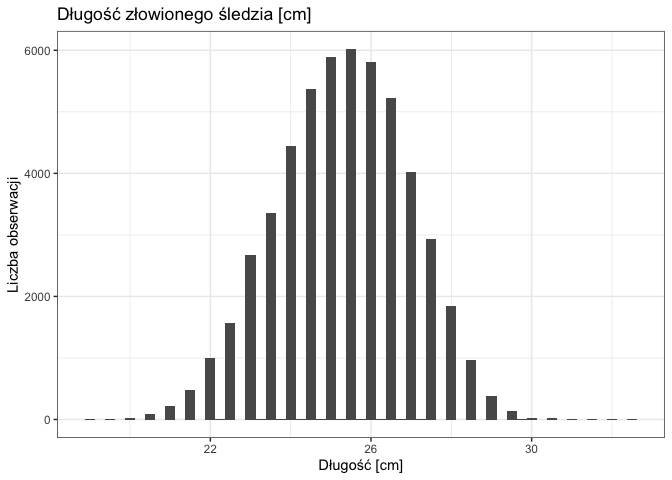
\includegraphics{Project_Herring_Analyze_files/figure-latex/cechy1-1.pdf}
Jak możemy zaobserwować, większość śledzi w połowie ma długość od 23 do
27 centymetrów.

\begin{Shaded}
\begin{Highlighting}[]
\NormalTok{plot_cfin1 <-}\StringTok{ }\KeywordTok{ggplot}\NormalTok{(content, }\KeywordTok{aes}\NormalTok{(}\DataTypeTok{x =}\NormalTok{ cfin1)) }\OperatorTok{+}\StringTok{ }\KeywordTok{geom_histogram}\NormalTok{(}\DataTypeTok{binwidth =} \FloatTok{1.0}\NormalTok{) }\OperatorTok{+}
\StringTok{  }\KeywordTok{theme_bw}\NormalTok{() }\OperatorTok{+}\StringTok{ }\KeywordTok{ggtitle}\NormalTok{(}\StringTok{'Calanus finmarchicus gat. 1'}\NormalTok{) }\OperatorTok{+}\StringTok{ }
\StringTok{  }\KeywordTok{xlab}\NormalTok{(}\KeywordTok{sprintf}\NormalTok{(}\StringTok{'Zagęszczenie planktonu [j]'}\NormalTok{)) }\OperatorTok{+}\StringTok{ }\KeywordTok{ylab}\NormalTok{(}\StringTok{'Liczba obserwacji'}\NormalTok{)}

\NormalTok{plot_cfin2 <-}\StringTok{ }\KeywordTok{ggplot}\NormalTok{(content, }\KeywordTok{aes}\NormalTok{(}\DataTypeTok{x =}\NormalTok{ cfin2)) }\OperatorTok{+}\StringTok{ }\KeywordTok{geom_histogram}\NormalTok{(}\DataTypeTok{binwidth =} \FloatTok{1.0}\NormalTok{) }\OperatorTok{+}
\StringTok{  }\KeywordTok{theme_bw}\NormalTok{() }\OperatorTok{+}\StringTok{ }\KeywordTok{ggtitle}\NormalTok{(}\StringTok{'Calanus finmarchicus gat. 2'}\NormalTok{) }\OperatorTok{+}\StringTok{ }
\StringTok{  }\KeywordTok{xlab}\NormalTok{(}\KeywordTok{sprintf}\NormalTok{(}\StringTok{'Zagęszczenie planktonu [j]'}\NormalTok{)) }\OperatorTok{+}\StringTok{ }\KeywordTok{ylab}\NormalTok{(}\StringTok{'Liczba obserwacji'}\NormalTok{)}

\KeywordTok{grid.arrange}\NormalTok{(plot_cfin1, plot_cfin2, }\DataTypeTok{nrow =} \DecValTok{1}\NormalTok{)}
\end{Highlighting}
\end{Shaded}

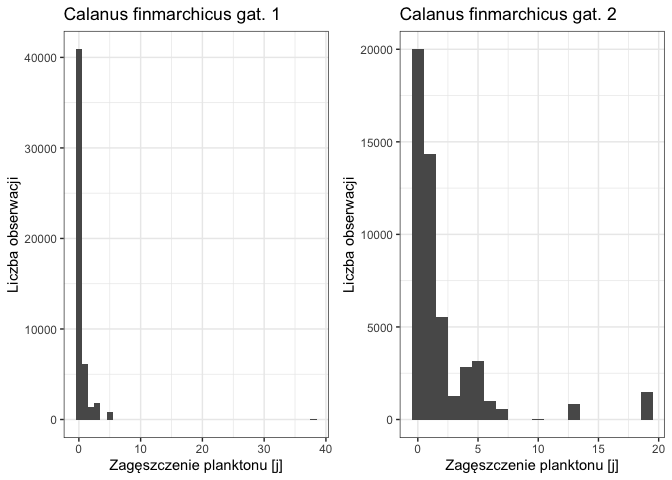
\includegraphics{Project_Herring_Analyze_files/figure-latex/cechy2-1.pdf}

\begin{Shaded}
\begin{Highlighting}[]
\NormalTok{plot_chel1 <-}\StringTok{ }\KeywordTok{ggplot}\NormalTok{(content, }\KeywordTok{aes}\NormalTok{(}\DataTypeTok{x =}\NormalTok{ chel1)) }\OperatorTok{+}\StringTok{ }\KeywordTok{geom_histogram}\NormalTok{(}\DataTypeTok{binwidth =} \FloatTok{0.5}\NormalTok{) }\OperatorTok{+}
\StringTok{  }\KeywordTok{theme_bw}\NormalTok{() }\OperatorTok{+}\StringTok{ }\KeywordTok{ggtitle}\NormalTok{(}\StringTok{'Calanus helgolandicus gat. 1'}\NormalTok{) }\OperatorTok{+}\StringTok{ }
\StringTok{  }\KeywordTok{xlab}\NormalTok{(}\KeywordTok{sprintf}\NormalTok{(}\StringTok{'Zagęszczenie planktonu [j]'}\NormalTok{)) }\OperatorTok{+}\StringTok{ }\KeywordTok{ylab}\NormalTok{(}\StringTok{'Liczba obserwacji'}\NormalTok{)}

\NormalTok{plot_chel2 <-}\StringTok{ }\KeywordTok{ggplot}\NormalTok{(content, }\KeywordTok{aes}\NormalTok{(}\DataTypeTok{x =}\NormalTok{ chel2)) }\OperatorTok{+}\StringTok{ }\KeywordTok{geom_histogram}\NormalTok{(}\DataTypeTok{binwidth =} \FloatTok{0.5}\NormalTok{) }\OperatorTok{+}
\StringTok{  }\KeywordTok{theme_bw}\NormalTok{() }\OperatorTok{+}\StringTok{ }\KeywordTok{ggtitle}\NormalTok{(}\StringTok{'Calanus helgolandicus gat. 2'}\NormalTok{) }\OperatorTok{+}\StringTok{ }
\StringTok{  }\KeywordTok{xlab}\NormalTok{(}\KeywordTok{sprintf}\NormalTok{(}\StringTok{'Zagęszczenie planktonu [j]'}\NormalTok{)) }\OperatorTok{+}\StringTok{ }\KeywordTok{ylab}\NormalTok{(}\StringTok{'Liczba obserwacji'}\NormalTok{)}

\KeywordTok{grid.arrange}\NormalTok{(plot_chel1, plot_chel2, }\DataTypeTok{nrow =} \DecValTok{1}\NormalTok{)}
\end{Highlighting}
\end{Shaded}

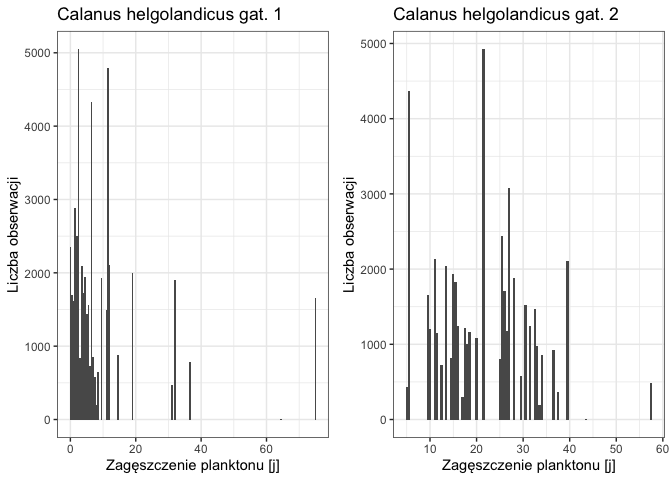
\includegraphics{Project_Herring_Analyze_files/figure-latex/cechy3-1.pdf}

\begin{Shaded}
\begin{Highlighting}[]
\NormalTok{plot_lcop1 <-}\StringTok{ }\KeywordTok{ggplot}\NormalTok{(content, }\KeywordTok{aes}\NormalTok{(}\DataTypeTok{x =}\NormalTok{ lcop1)) }\OperatorTok{+}\StringTok{ }\KeywordTok{geom_histogram}\NormalTok{(}\DataTypeTok{binwidth =} \FloatTok{0.5}\NormalTok{) }\OperatorTok{+}
\StringTok{  }\KeywordTok{theme_bw}\NormalTok{() }\OperatorTok{+}\StringTok{ }\KeywordTok{ggtitle}\NormalTok{(}\StringTok{'Widłonogi gat. 1'}\NormalTok{) }\OperatorTok{+}\StringTok{ }
\StringTok{  }\KeywordTok{xlab}\NormalTok{(}\KeywordTok{sprintf}\NormalTok{(}\StringTok{'Zagęszczenie planktonu [j]'}\NormalTok{)) }\OperatorTok{+}\StringTok{ }\KeywordTok{ylab}\NormalTok{(}\StringTok{'Liczba obserwacji'}\NormalTok{)}

\NormalTok{plot_lcop2 <-}\StringTok{ }\KeywordTok{ggplot}\NormalTok{(content, }\KeywordTok{aes}\NormalTok{(}\DataTypeTok{x =}\NormalTok{ lcop2)) }\OperatorTok{+}\StringTok{ }\KeywordTok{geom_histogram}\NormalTok{(}\DataTypeTok{binwidth =} \FloatTok{0.5}\NormalTok{) }\OperatorTok{+}
\StringTok{  }\KeywordTok{theme_bw}\NormalTok{() }\OperatorTok{+}\StringTok{ }\KeywordTok{ggtitle}\NormalTok{(}\StringTok{'Widłonogi gat. 2'}\NormalTok{) }\OperatorTok{+}\StringTok{ }
\StringTok{  }\KeywordTok{xlab}\NormalTok{(}\KeywordTok{sprintf}\NormalTok{(}\StringTok{'Zagęszczenie planktonu [j]'}\NormalTok{)) }\OperatorTok{+}\StringTok{ }\KeywordTok{ylab}\NormalTok{(}\StringTok{'Liczba obserwacji'}\NormalTok{)}

\KeywordTok{grid.arrange}\NormalTok{(plot_lcop1, plot_lcop2, }\DataTypeTok{nrow =} \DecValTok{1}\NormalTok{)}
\end{Highlighting}
\end{Shaded}

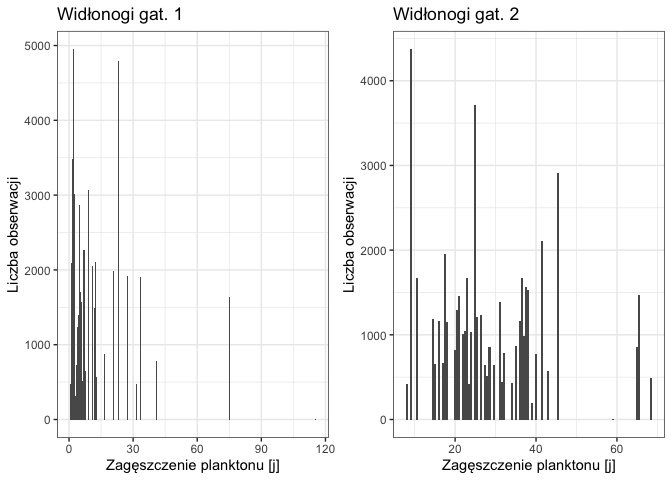
\includegraphics{Project_Herring_Analyze_files/figure-latex/cechy4-1.pdf}

\begin{Shaded}
\begin{Highlighting}[]
\NormalTok{plot_fbar <-}\StringTok{ }\KeywordTok{ggplot}\NormalTok{(content, }\KeywordTok{aes}\NormalTok{(}\DataTypeTok{x =}\NormalTok{ fbar)) }\OperatorTok{+}\StringTok{ }\KeywordTok{geom_histogram}\NormalTok{(}\DataTypeTok{binwidth =} \FloatTok{0.05}\NormalTok{) }\OperatorTok{+}
\StringTok{  }\KeywordTok{theme_bw}\NormalTok{() }\OperatorTok{+}\StringTok{ }\KeywordTok{ggtitle}\NormalTok{(}\StringTok{'Natężenie połowów') + }
\StringTok{  xlab(sprintf('}\NormalTok{Ułamek pozostawionego narybku}\StringTok{')) + ylab('}\NormalTok{Liczba obserwacji}\StringTok{')}

\StringTok{plot_recr <- ggplot(content, aes(x = recr)) + geom_histogram(binwidth = 50000.0) +}
\StringTok{  theme_bw() + ggtitle('}\NormalTok{Roczny narybek}\StringTok{') + }
\StringTok{  xlab(sprintf('}\NormalTok{Liczba śledzi}\StringTok{')) + ylab('}\NormalTok{Liczba obserwacji}\StringTok{')}

\StringTok{plot_cumf <- ggplot(content, aes(x = cumf)) + geom_histogram(binwidth = 0.02) +}
\StringTok{  theme_bw() + ggtitle('}\NormalTok{Łączne roczne natężenie połowów') }\OperatorTok{+}\StringTok{ }
\StringTok{  }\KeywordTok{xlab}\NormalTok{(}\KeywordTok{sprintf}\NormalTok{(}\StringTok{'Ułamek pozostawionego narybku'}\NormalTok{)) }\OperatorTok{+}\StringTok{ }\KeywordTok{ylab}\NormalTok{(}\StringTok{'Liczba obserwacji'}\NormalTok{)}

\NormalTok{plot_totaln <-}\StringTok{ }\KeywordTok{ggplot}\NormalTok{(content, }\KeywordTok{aes}\NormalTok{(}\DataTypeTok{x =}\NormalTok{ totaln)) }\OperatorTok{+}\StringTok{ }\KeywordTok{geom_histogram}\NormalTok{(}\DataTypeTok{binwidth =} \FloatTok{1000.0}\NormalTok{) }\OperatorTok{+}
\StringTok{  }\KeywordTok{theme_bw}\NormalTok{() }\OperatorTok{+}\StringTok{ }\KeywordTok{ggtitle}\NormalTok{(}\StringTok{'Łączna liczba złowionych ryb'}\NormalTok{) }\OperatorTok{+}\StringTok{ }
\StringTok{  }\KeywordTok{xlab}\NormalTok{(}\KeywordTok{sprintf}\NormalTok{(}\StringTok{'Liczba śledzi'}\NormalTok{)) }\OperatorTok{+}\StringTok{ }\KeywordTok{ylab}\NormalTok{(}\StringTok{'Liczba obserwacji'}\NormalTok{)}

\KeywordTok{grid.arrange}\NormalTok{(plot_fbar, plot_recr, plot_cumf, plot_totaln, }\DataTypeTok{nrow =} \DecValTok{2}\NormalTok{)}
\end{Highlighting}
\end{Shaded}

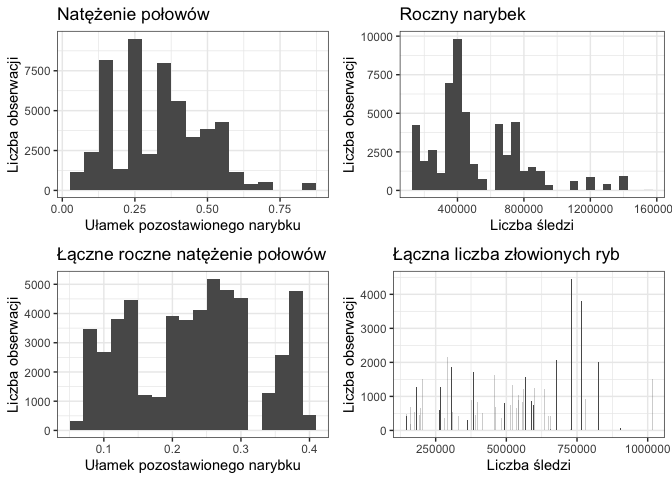
\includegraphics{Project_Herring_Analyze_files/figure-latex/cechy5-1.pdf}

\begin{Shaded}
\begin{Highlighting}[]
\NormalTok{plot_sst <-}\StringTok{ }\KeywordTok{ggplot}\NormalTok{(content, }\KeywordTok{aes}\NormalTok{(}\DataTypeTok{x =}\NormalTok{ sst)) }\OperatorTok{+}\StringTok{ }\KeywordTok{geom_histogram}\NormalTok{(}\DataTypeTok{binwidth =} \FloatTok{0.1}\NormalTok{) }\OperatorTok{+}
\StringTok{  }\KeywordTok{theme_bw}\NormalTok{() }\OperatorTok{+}\StringTok{ }\KeywordTok{ggtitle}\NormalTok{(}\StringTok{'Temperatura przy powierzchni wody'}\NormalTok{) }\OperatorTok{+}\StringTok{ }
\StringTok{  }\KeywordTok{xlab}\NormalTok{(}\KeywordTok{sprintf}\NormalTok{(}\StringTok{'Temperatura'}\NormalTok{)) }\OperatorTok{+}\StringTok{ }\KeywordTok{ylab}\NormalTok{(}\StringTok{'Liczba obserwacji'}\NormalTok{)}

\NormalTok{plot_sal <-}\StringTok{ }\KeywordTok{ggplot}\NormalTok{(content, }\KeywordTok{aes}\NormalTok{(}\DataTypeTok{x =}\NormalTok{ sal)) }\OperatorTok{+}\StringTok{ }\KeywordTok{geom_histogram}\NormalTok{(}\DataTypeTok{binwidth =} \FloatTok{0.01}\NormalTok{) }\OperatorTok{+}
\StringTok{  }\KeywordTok{theme_bw}\NormalTok{() }\OperatorTok{+}\StringTok{ }\KeywordTok{ggtitle}\NormalTok{(}\StringTok{'Poziom zasolenia wody'}\NormalTok{) }\OperatorTok{+}\StringTok{ }
\StringTok{  }\KeywordTok{xlab}\NormalTok{(}\KeywordTok{sprintf}\NormalTok{(}\StringTok{'Zasolenie wody'}\NormalTok{)) }\OperatorTok{+}\StringTok{ }\KeywordTok{ylab}\NormalTok{(}\StringTok{'Liczba obserwacji'}\NormalTok{)}

\NormalTok{plot_xmonth <-}\StringTok{ }\KeywordTok{ggplot}\NormalTok{(content, }\KeywordTok{aes}\NormalTok{(}\DataTypeTok{x =}\NormalTok{ xmonth)) }\OperatorTok{+}\StringTok{ }\KeywordTok{geom_histogram}\NormalTok{(}\DataTypeTok{binwidth =} \FloatTok{0.5}\NormalTok{) }\OperatorTok{+}
\StringTok{  }\KeywordTok{theme_bw}\NormalTok{() }\OperatorTok{+}\StringTok{ }\KeywordTok{ggtitle}\NormalTok{(}\StringTok{'Miesic połowu'}\NormalTok{) }\OperatorTok{+}\StringTok{ }
\StringTok{  }\KeywordTok{xlab}\NormalTok{(}\KeywordTok{sprintf}\NormalTok{(}\StringTok{'Miesiąc'}\NormalTok{)) }\OperatorTok{+}\StringTok{ }\KeywordTok{ylab}\NormalTok{(}\StringTok{'Liczba obserwacji'}\NormalTok{)}

\NormalTok{plot_nao <-}\StringTok{ }\KeywordTok{ggplot}\NormalTok{(content, }\KeywordTok{aes}\NormalTok{(}\DataTypeTok{x =}\NormalTok{ nao)) }\OperatorTok{+}\StringTok{ }\KeywordTok{geom_histogram}\NormalTok{(}\DataTypeTok{binwidth =} \FloatTok{0.5}\NormalTok{) }\OperatorTok{+}
\StringTok{  }\KeywordTok{theme_bw}\NormalTok{() }\OperatorTok{+}\StringTok{ }\KeywordTok{ggtitle}\NormalTok{(}\StringTok{'Oscylacja północnoatlantycka'}\NormalTok{) }\OperatorTok{+}\StringTok{ }
\StringTok{  }\KeywordTok{xlab}\NormalTok{(}\KeywordTok{sprintf}\NormalTok{(}\StringTok{'Oscylacja'}\NormalTok{)) }\OperatorTok{+}\StringTok{ }\KeywordTok{ylab}\NormalTok{(}\StringTok{'Liczba obserwacji'}\NormalTok{)}

\KeywordTok{grid.arrange}\NormalTok{(plot_sst, plot_sal, plot_xmonth, plot_nao, }\DataTypeTok{nrow =} \DecValTok{2}\NormalTok{)}
\end{Highlighting}
\end{Shaded}

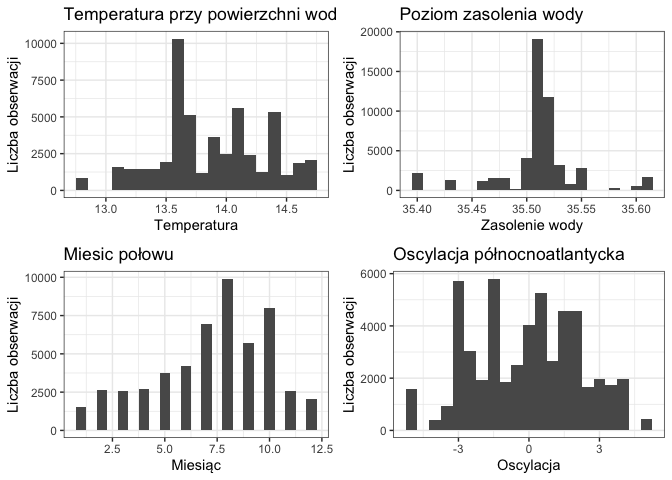
\includegraphics{Project_Herring_Analyze_files/figure-latex/cechy6-1.pdf}

Analizując przedstawione wykresy dotyczące poszczególnych atrybutów
opisujących połowy możemy zaobserwować rozkład zbliżony do normalnego
dla wielu z nich (chociażby parametr długości śledzia). W przypadku
parametrów dostępności planktonu \emph{Calanus finmarchicus gat. 1} oraz
\emph{Widłonogów gat. 1} obserwujemy występowanie drobnej próbki danych
odbierających znacząco od reszty. Na potrzeby dalszego przetwarzania
dane zostaną oczyszczone z tych obserwacji odstających.

\begin{Shaded}
\begin{Highlighting}[]
\NormalTok{without_outliers =}
\StringTok{  }\NormalTok{content }\OperatorTok
\StringTok{  }\KeywordTok{filter}\NormalTok{(cfin1 }\OperatorTok{<=}\StringTok{ }\DecValTok{10} \OperatorTok{|}\StringTok{ }\KeywordTok{is.na}\NormalTok{(cfin1)) }\OperatorTok
\StringTok{  }\KeywordTok{filter}\NormalTok{(lcop1 }\OperatorTok{<=}\StringTok{ }\DecValTok{90} \OperatorTok{|}\StringTok{ }\KeywordTok{is.na}\NormalTok{(lcop1))}
\end{Highlighting}
\end{Shaded}

Po operacji w zbiorze obserwacji pozostało 52576 próbek (usunięto 6
obserwacji).

\begin{Shaded}
\begin{Highlighting}[]
\NormalTok{plot_cfin1_clear <-}\StringTok{ }\KeywordTok{ggplot}\NormalTok{(without_outliers, }\KeywordTok{aes}\NormalTok{(}\DataTypeTok{x =}\NormalTok{ cfin1)) }\OperatorTok{+}\StringTok{ }\KeywordTok{geom_histogram}\NormalTok{(}\DataTypeTok{binwidth =} \FloatTok{1.0}\NormalTok{) }\OperatorTok{+}
\StringTok{  }\KeywordTok{theme_bw}\NormalTok{() }\OperatorTok{+}\StringTok{ }\KeywordTok{ggtitle}\NormalTok{(}\StringTok{'Calanus finmarchicus gat. 1'}\NormalTok{) }\OperatorTok{+}\StringTok{ }
\StringTok{  }\KeywordTok{xlab}\NormalTok{(}\KeywordTok{sprintf}\NormalTok{(}\StringTok{'Zagęszczenie planktonu [j]'}\NormalTok{)) }\OperatorTok{+}\StringTok{ }\KeywordTok{ylab}\NormalTok{(}\StringTok{'Liczba obserwacji'}\NormalTok{)}

\NormalTok{plot_lcop1_clear <-}\StringTok{ }\KeywordTok{ggplot}\NormalTok{(without_outliers, }\KeywordTok{aes}\NormalTok{(}\DataTypeTok{x =}\NormalTok{ lcop1)) }\OperatorTok{+}\StringTok{ }\KeywordTok{geom_histogram}\NormalTok{(}\DataTypeTok{binwidth =} \FloatTok{0.5}\NormalTok{) }\OperatorTok{+}
\StringTok{  }\KeywordTok{theme_bw}\NormalTok{() }\OperatorTok{+}\StringTok{ }\KeywordTok{ggtitle}\NormalTok{(}\StringTok{'Widłonogi gat. 1'}\NormalTok{) }\OperatorTok{+}\StringTok{ }
\StringTok{  }\KeywordTok{xlab}\NormalTok{(}\KeywordTok{sprintf}\NormalTok{(}\StringTok{'Zagęszczenie planktonu [j]'}\NormalTok{)) }\OperatorTok{+}\StringTok{ }\KeywordTok{ylab}\NormalTok{(}\StringTok{'Liczba obserwacji'}\NormalTok{)}

\KeywordTok{grid.arrange}\NormalTok{(plot_cfin1_clear, plot_lcop1_clear, }\DataTypeTok{nrow =} \DecValTok{1}\NormalTok{)}
\end{Highlighting}
\end{Shaded}

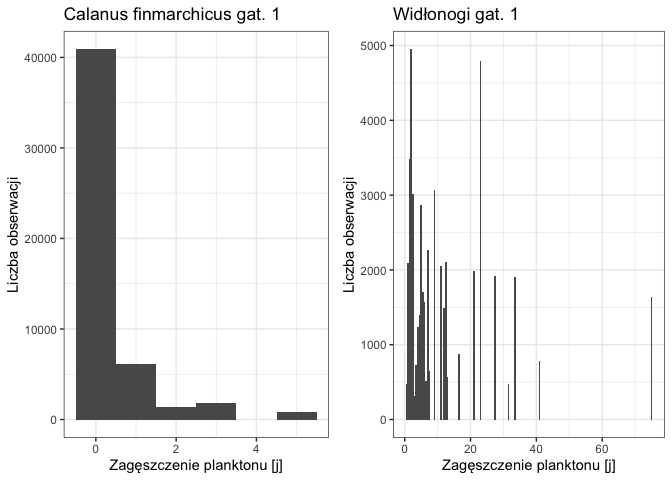
\includegraphics{Project_Herring_Analyze_files/figure-latex/cechy7-1.pdf}

\hypertarget{przetwarzanie-brakujux105cych-danych}{%
\section{Przetwarzanie brakujących
danych}\label{przetwarzanie-brakujux105cych-danych}}

TODO: Analiza jakie atrybuty oraz liczność TODO: Uśrednienie wartości
bazując na rozkładzie


\end{document}
